\subsection{Sequence-to-SQL}

\subsubsection{Seq2Seq}

The seq2seq model\cite{DBLP:journals/corr/SutskeverVL14} is a type of neural network architecture that has revolutionized the field of natural language processing. It generates meaningful sequences from input data, such as translating one language into another or summarizing text. The primary components of the seq2seq model are an encoder and decoder, which work together to learn how to map inputs onto outputs in a way that preserves their meaning.

The encoder takes raw input data and converts it into a series of numerical vectors known as embeddings. These embeddings represent each word or phrase in the input sequence with its unique vector representation so that it can be understood by the decoder for further processing. The decoder then uses these representations and other parameters like attention weights and recurrent layers to generate output sequences based on what was learned during training time from previous examples given by humans or machines alike.

Seq2Seq models can be trained using techniques such as supervised learning, which is trained on a dataset of input-output pairs, or unsupervised learning, where the model is trained to reconstruct the input sequence. Attention mechanisms, such as the attention mechanism used in the Transformer model, can also be incorporated into Seq2Seq models to improve their performance by allowing the decoder to focus selectively on certain parts of the input sequence.

Finally, once appropriately trained on large datasets containing millions of examples across multiple languages (or even within just one), this powerful tool can be used for tasks such as machine translation between two different languages; automatically generating summaries; question-answering systems; voice recognition software; among many others! Seq2Seq models have become increasingly popular due to their ability to quickly process large volumes of information while still maintaining accuracy and efficiency when compared to traditional methods like rule-based algorithms. However, one of the significant challenges of Seq2Seq models is the risk of generating irrelevant or nonsensical outputs, known as the "exposure bias" problem. Researchers have proposed various solutions to this problem, such as using beam search during decoding.

% image of seq2seq.png
\begin{figure}[ht]
    \centering
    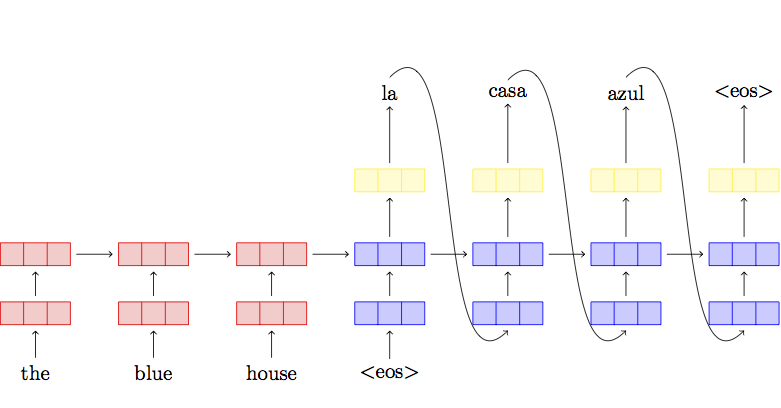
\includegraphics[width=0.5\textwidth]{pics/seq2seq.png}
    \caption{Example of Seq2Seq model in translating a sentence from English to French.\cite{DBLP:journals/corr/SutskeverVL14}}
    \label{fig:seq2seq}
\end{figure}

\subsubsection{Seq2SQL}

Seq2SQL \cite{zhong_seq2sql_2017} is a deep-learning system based on a straightforward concept: similar to Seq2Seq\cite{DBLP:journals/corr/SutskeverVL14}, it takes an input sentence or phrase, breaks it down into its components, and maps them onto a SQL query structure. Seq2SQL was one of the first deep-learning systems to employ this approach. However, later systems opted for different approaches due to the significant disadvantage of this approach: it does not consider the strict grammar rules of SQL when generating queries, making it the most error-prone. On the other hand, sequence-to-sequence architectures may have the potential to provide more accurate results but require more complex architectures to be implemented.

As part of this model, its authors released the WikiSQL dataset, which ushered in a new era of text-to-SQL deep learning research. With a seq-to-seq network, the system predicts the aggregation function and the column for the SELECT clause. Its major drawback is that it generates parts of the query that can lead to syntactic errors.